\chapter{Deterministic annealing}

\section{The problem of centroid-based cluster-
ing}
\label{sec:problem}

In this chapter, we consider the problem of centroid-based clustering. In
this problem, an observation is a sample $X = \{x_1, \ldots, x_N\} \subseteq \mathbb{R}^d$ of points
and our objective is to compute a set $\{\theta_1, \ldots, \theta_K\} \subseteq \mathbb{R}^d$ of $K$ centroids and a \emph{cluster assignment} function $c : \{1, \ldots, N\} \to \{1, \ldots, K\}$, where $K \in \mathbb{N}$ is a hyperparameter.
We let the hypothesis class $\mathcal{C}$ be all possible cluster assignment functions with fixed $K$.

As cost function, we choose the $K$-means cost function:
%
\begin{equation}
R(c, \theta, X) := \sum_{i \leq n} \left\|x_i - \theta_{c(i)}\right\|^2.
\label{eq:k_means_cost_fun}
\end{equation}
%
Note that, in contrast to $K$-means, we neither require $\theta_k$ to be the mean of all points in $X$ assigned to cluster $k$ nor that $c(x)$ is the index of the centroid closest to $x$.

\section{Chapter outline}
\label{sec:chapter_outline}

In this chapter, we study how to apply simulated annealing to the problem
of clustering, and derive a simplified version called deterministic annealing, proposed by Kenneth Rose~\cite{rose1998deterministic}. We compare deterministic annealing
against a popular ERM approach, $K$-means, and empirically show that deterministic annealing often provides solutions that generalize better than
$K$-means. Furthermore, combining deterministic annealing with posterior
agreement gives a method to estimate the number of clusters while executing
deterministic annealing.

\subsection*{Deterministic annealing}

Deterministic annealing originates from applying simulated annealing to
clustering. We can summarize simulated annealing in this context in the
following three steps.

\begin{enumerate}
\item Pick a first model $c$ and an initial (high) temperature.
\item Use MCMC to draw a sample from $p(\cdot \mid X)$, the Gibbs distribution induced by $R(\cdot, \cdot, X)$, starting from $c$ as the first model in the sample.
\item Decrease the temperature, let $c$ be the last model in the MCMC
sample, and go to Step 2.
\end{enumerate}

We see in Section \ref{sec:gibbs_factorizes_da} that the Gibbs distribution induced by the cost
function $R(\cdot, \cdot, X)$ is actually tractable. This means that we do not need to do MCMC sampling. We can instead directly computing the Gibbs distribution. The three steps become the following procedure, called \emph{deterministic annealing}:
%
\begin{enumerate}
\item Pick an initial set of centroids and an initial (high) temperature.
\item Compute the Gibbs distribution $p(\cdot \mid X)$, for $\theta$ arbitrary.
\item Decrease the temperature and go to Step 2.
\end{enumerate}
%
In Section~\ref{sec:computing_centroids_da}, we show that the centroids can then be computed as those that maximize the Gibbs distribution's entropy. However, this maximization is intractable, so we use the EM algorithm to efficiently compute an approximation. We combine all these insights to formulate the algorithm for deterministic annealing in Section~\ref{sec:algo_da}.

In Section~\ref{sec:experiments}, we provide some experimental results comparing deterministic annealing against $K$-means. 

In Section~\ref{sec:phase_transition}, we describe an interesting behavior of deterministic annealing.
When the temperature is high, there is only one cluster containing
all points and whose centroid is just the sample mean. As the temperature
decreases, this cluster decomposes into several clusters that continue
to decompose as the temperature keeps decreasing. One could argue that
at a sufficiently low temperature, each point becomes its own cluster.

Finally, in Section~\ref{sec:da_pa}, we exploit this behavior and posterior agreement to determine the number of clusters while executing deterministic annealing. This yields an extra advantage of deterministic annealing over other standard clustering methods like $K$-means which demand to set the number of clusters in advance.

\section{Tractability of the Gibbs distribution}
\label{sec:gibbs_factorizes_da}

We assume that our hypothesis class $\mathcal{C}$ is the set of all cluster assignments $c : \{1, \ldots, N\} \to \{1, \ldots, K\}$.\todo{Observe that $c$'s domain must be the set of numbers up to $N$ and not an Euclidean domain. Otherwise, the Gibbs distribution is a continuous distribution!} We define then the family of Gibbs distributions
induced by the $K$-means cost function as all distributions over $\mathcal{C}$ of the
form
%
\begin{equation}
p(\cdot \mid \theta, X) \propto \exp\left(-\frac{1}{T}R(c, \theta, X)\right).
\label{eq:gibbs_distr}
\end{equation}
%
Here, $T > 0$ is a hyper-parameter denoting the temperature and $\theta \in \mathbb{R}^{K \times d}$ are parameters denoting the cluster centroids. 

The centroids are chosen to be hyper-parameters just for convenience.
One could treat them as part of the hypothesis class, but this substantially complicates the analysis.

\begin{theorem}
A Gibbs distribution induced by the K-means cost function
factorizes as follows:
%
\begin{equation}
p(c \mid \theta, X) = \prod_{i \leq N} p(c(i) \mid \theta, X),
\label{eq:gibbs_distr_factorizes}
\end{equation}
%
where
%
\begin{equation}
p(c(i) \mid \theta, X) \propto \exp\left(-\frac{1}{T}\left\|x_i - \theta_{c(i)}\right\|^2\right).
\label{eq:gibbs_factors_da}
\end{equation}
%
\label{thm:gibbs_factorizes}
\end{theorem}

\begin{proof}
The Gibbs distribution is
%
\begin{equation}
p(c \mid \theta, X) = \frac{\exp\left(- \frac{1}{T}\sum_{i \leq N}\left\|x_i - \theta_{c(i)}\right\|^2\right)}{\sum_{c \in \mathcal{C}}\exp\left(- \frac{1}{T}\sum_{i \leq N}\left\|x_i - \theta_{c(i)}\right\|^2\right)}.
\end{equation}

The numerator can be rewritten as follows:
%
\begin{equation}
\exp\left(- \frac{1}{T}\sum_{i \leq N}\left\|x_i - \theta_{c(i)}\right\|^2\right) = \prod_{i \leq N}\exp\left(- \frac{1}{T}\left\|x_i - \theta_{c(i)}\right\|^2\right).
\end{equation}

We now apply the combinatorial trick that we studied in the lecture
to rewrite the denominator. Unfortunately, I do not see a better way to explain this trick without the diagrams from the lecture.
%
\begin{equation}
\sum_{c \in \mathcal{C}} \exp\left(- \frac{1}{T}\sum_{i \leq N}\left\|x_i - \theta_{c(i)}\right\|^2\right) = \ldots = \prod_{i \leq N} \sum_{k \leq K} \exp\left(-\frac{1}{T}\left\|x_i = \theta_i\right\|^2\right).
\end{equation}

Putting these results together yields that
%
\begin{align}
p(c \mid \theta, X) &= \frac{\prod_{i \leq N}\exp\left(- \frac{1}{T}\left\|x_i - \theta_{c(i)}\right\|^2\right)}{\prod_{i \leq N}\sum_{k \leq K}\exp\left(- \frac{1}{T}\left\|x_i - \theta_{k}\right\|^2\right)}\\
&= \prod_{i \leq N}\frac{\exp\left(- \frac{1}{T}\left\|x_i - \theta_{c(i)}\right\|^2\right)}{\sum_{k \leq K}\exp\left(- \frac{1}{T}\left\|x_i - \theta_{k}\right\|^2\right)}\\
&= \prod_{i \leq N}p(c(i) \mid \theta, X).
\end{align}
\end{proof} 

Theorem~\ref{thm:gibbs_factorizes} shows that we can compute $p(c \mid \theta, X)$ in just $O(NK)$-time.
You just have to compute $\exp\left(- \frac{1}{T}\left\|x_i - \theta_k\right\|^2\right)$, which is $O(1)$-time, for $i \leq N$ and $k \leq K$. Hence, computing $p(c(i) \mid \theta, X)$ takes $O(K)$-time, for $i \leq N$, yielding a total computing time of $O(NK)$.

\section{Computing the centroids}
\label{sec:computing_centroids_da}

The calculations from the previous section do not tell us the values of the centroids. Remember that we follow the maximum-entropy principle, so
we compute the centroids that maximize the entropy of $p(\cdot \mid \theta, X)$. In this
section, we use $C$ to denote a random cluster assignment whose distribution
is $p(\cdot \mid \theta, X)$.

We assume here that $\mathbb{E}_{C \sum p(\cdot \mid \theta, X)} = \mu$, for some fixed $\mu \in \mathbb{R}^+$ and that the temperature hyper-parameter
of $p(\cdot \mid \theta, X)$ depends exclusively on $\mu$.

\begin{lemma}
If, for a set $\theta^*$ of centroids,
%
\begin{equation}
\frac{\partial H \left[p(\cdot \mid \theta, X)\right]}{\partial \theta} \Bigr|_{\theta^*} = 0,
\end{equation}
%
then
%
\begin{equation}
\mathbb{E}_{C \sim p(\cdot \mid \theta, X)}\left[\frac{\partial}{\partial \theta}R(C, \theta, X)\Bigr|_{\theta^*}\right] = 0.
\end{equation}
\label{lem:stationarity_condition}
\end{lemma}

\begin{proof}
We leave the proof details as an exercise and provide just a vague
proof. For convenience, all expectations are with respect to a random cluster assignment $C \sim p(\cdot \mid \theta, X)$.

First, show that
%
\begin{equation}
H\left[p(\cdot \mid \theta, X)\right] = \frac{1}{T}\mathbb{E}\left[R(C, \theta, X)\right] + \mathbb{E}\left[\log \sum_{c \in \mathcal{C}} \exp\left(-\frac{1}{T}R(c, \theta, X)\right)\right].
\end{equation}

Recall that $\mathbb{E}\left[R(C, \theta, X)\right]$ is fixed to be constant, by construction. Hence,
the first term on the right-hand side of the equation above is constant with
respect to $\theta$. Moreover, the second term does not depend on the random variable $C$. We get then that
%
\begin{equation}
H[p(\cdot \mid \theta, X)] = \text{const} + \log \sum_{c \in \mathcal{C}} \exp\left(- \frac{1}{T}R(c, \theta, X)\right).
\end{equation}
%
Take the derivative with respect to on both sides and show that
%
\begin{equation}
\frac{\partial H[p\left(\cdot \mid \theta, X\right)]}{\partial \theta} = \mathbb{E}_{C \sim p(\cdot \mid \theta^*, X)} \left[\frac{\partial}{\partial \theta}R(C, \theta, X)\right].
\end{equation}
%
This equality yields the desired result.
\end{proof}

For an event $A$, we now denote by $\mathbf{1}{A}$ the indicator function. That is,
%
\begin{equation}
\mathbf{1}{A}(\omega)
\begin{cases}
1 & \text{if $\omega \in A$ and}\\
0 & \text{otherwise}.
\end{cases}
\end{equation}
%

\begin{lemma}
Let $C$ denote a random cluster assignment and $C(i)$, for $i \leq N$,
the cluster that $C$ assigns to $x_i$. If $R(\cdot, \cdot, X)$ is the $K$-means cost function, then
%
\begin{equation}
\frac{\partial}{\partial \theta_k} R(C, \theta, X) = 2\theta_k \sum_{i \leq N} \mathbf{1}\left\{C(i) = k\right\} - 2\sum_{i \leq N} x_i \mathbf{1}\left\{C(i) = k\right\}.
\label{eq:deriv_cost_fun_da}
\end{equation}
%
\end{lemma}

\begin{proof}
The proof is a straightforward use of vector calculus and is left as
an exercise.
\end{proof}

\begin{theorem}
The set $\theta^*$ of centroids that maximize the entropy of $p(\cdot \mid \theta, X)$ must satisfy the following conditions.
%
\begin{equation}
\theta^*_k = \frac{\sum_{i \leq N} x_i \prob\left(C(i) = k \mid \theta^*, X\right)}{\sum_{i \leq N} \prob\left(C(i) = k \mid \theta^*, X\right)},\text{ for $k \leq K$},
\label{eq:thm_stationarity_conds_centroids_da}
\end{equation}
%
where
%
\begin{equation}
\prob\left(C(i) = k \mid \theta^*, X\right) \propto \exp\left(- \frac{1}{T}\left\|x_i - \theta^*_k\right\|^2\right).
\end{equation}
%
\end{theorem}

\begin{proof}
If $\theta^*$ maximizes the entropy of $p(\cdot \mid \theta, X)$, then, by Lemma~\ref{lem:stationarity_condition},
%
\begin{equation}
\mathbb{E}_{C \sim p(\cdot \mid \theta^*, X)}\left[\frac{\partial}{\partial \theta} R(C, \theta, X)\Bigr|_{\theta^*}\right] = 0.
\end{equation}

Plugging Equation~\ref{eq:deriv_cost_fun_da} in the equation above yields that
%
\begin{equation}
\mathbb{E}_{C \sim p(\cdot \mid \theta^*, X)}\left[\theta^*_k \sum_{i \leq N} \mathbf{1}\left\{C(i) = k\right\} - \sum_{i \leq N} x_i \mathbf{1}\left\{C(i) = k\right\}\right] = 0.
\end{equation}
%
Apply now linearity of the expectation and the fact that $\mathbb{E}\left[\mathbf{1}A\right] = \prob\left(A\right)$ to get that
%
\begin{equation}
\theta^*_k \sum_{i \leq N} \prob\left(C(i) = k \mid \theta^*, X\right) - \sum_{i \leq N}x_i \prob\left(C(i) = k \mid \theta^*, X\right) = 0.
\end{equation}

The desired condition follows from this equation.
\end{proof}

Unfortunately, Equation~\ref{eq:thm_stationarity_conds_centroids_da} does not give us a closed formula to compute $\theta^*$. We can still attempt to estimate $\theta^*$ iteratively, with the following
procedure.

\begin{enumerate}
\item Set $t \gets 0$ and $\theta^*_t$ to an arbitrary value.
\item Set $t \gets t + 1$ and
%
\begin{equation}
\theta^*_{t+1} \gets \frac{\sum_{i \leq N} \prob\left(C(i) = k \mid \theta^*_t, X\right)x_i}{\prob\left(C(i) = k \mid \theta^*_t, X\right)}.
\end{equation}
%
This procedure converges to a local maximum of $H[p(\cdot \mid \theta, X)]$.
\end{enumerate}

\begin{exercise}
Demonstrate that the procedure above also results from applying
the EM-algorithm to the following maximization problem:
%
\begin{equation}
\max_{\theta} \log \sum_{c \in \mathcal{C}} p(X, c \mid \theta),
\end{equation}
%
where $p(X, c \mid \theta) := p(c \mid \theta, X)p(X)$ and $p(X)$ is the pdf of the phenomenon where $X$ comes from. Use this to demonstrate why the procedure above
converges.
\end{exercise}

\section{Deterministic annealing}
\label{sec:algo_da}

We now collect all insights from this chapter and use them to propose
an improved version of simulated annealing, called \emph{deterministic annealing}.
Algorithm~\ref{algo:da_algo_da} provides the details. The idea of this procedure is the
following.

\begin{enumerate}
\item We set a high value for the temperature and start with arbitrary
centroids.
\item \label{step:em_alternation} We alternate between (i) computing the maximum-entropy distribution
for a random cluster assignment while fixing the centroids
and (ii) computing the centroids that maximize the entropy of that
distribution. This alternation is repeated until convergence of the
centroids.
\item We reduce the temperature and repeat Step~\ref{step:em_alternation}. To avoid having repeated
centroids, we add a small amount of noise.
\end{enumerate}

We remark some differences between deterministic annealing and simulated
annealing:

\begin{itemize}
\item There is no MCMC sampling. This is because the Gibbs distribution
induced by the $K$-means cost is tractable. So we can just compute it
directly.
\item The centroids are treated as parameters of the Gibbs distribution
and not as part of the hypothesis class. This is done mainly for
convenience. A Gibbs distribution that also treats the centroids as
random variables makes the whole procedure intractable.
\end{itemize}

\begin{algorithm}
\begin{algorithmic}[1]
\State Let
\State \qquad $\epsilon > 0$ be a temperature threshold,
\State \qquad $\texttt{reduce}(\cdot)$ be a function for decreasing the temperature.
\State \qquad $\texttt{close}\left(\cdot, \cdot\right)$ be a function that evaluates if two matrices are close.
\Function{DetAnn}{$\epsilon$, \texttt{reduce}, \texttt{close}}
\State $T \gets \infty$ \Comment{$\infty$ is a sufficiently large value.}
\State $\theta \gets \$$ \Comment{Define arbitrary initial centroids.}
\While{$T > \epsilon$}
\Repeat
\State $\theta_0 \gets \theta$
\State Compute $\prob\left(C(i) = k \mid \theta_0, X\right)$, for $i \leq N$ and $k \leq K$
\State $\displaystyle \theta \gets \frac{\sum_{i \leq N} \prob\left(C(i) = k \mid \theta_0, X\right) x_i}{\sum_{i \leq N} \prob\left(C(i) = k \mid \theta_0, X\right)}$
\Until{$\texttt{close}\left(\theta, \theta_0\right)$}
\State Add a small amount of noise to each centroid in $\theta$.
\State $T \gets \texttt{reduce}(T)$
\EndWhile
\State \textbf{return} $\theta$, $\{\prob\left(C(i) = k \mid \theta, X\right) \mid i \leq N, k \leq K\}$
\EndFunction
\end{algorithmic}
\caption{Deterministic annealing}
\label{algo:da_algo_da}
\end{algorithm}

\section{Experimental results}
\label{sec:experiments}

Figure~\ref{fig:da_vs_kmeans}, from Rose~\cite{rose1991deterministic, rose1998deterministic}, compares deterministic annealing with $K$-means
on a particular dataset $X$ which is a sample from a mixture of six Gaussians
with different means and different covariance matrices. $K$-means depends
on the initialization, so it was run 25 times. The result shown in the
figure was obtained only once, and in more than 80\% of the runs, $K$-
means was stuck in a local minimum. In contrast, deterministic annealing
is independent of the initialization and finds the global minimum more
often than $K$-means. For both $K$-means and deterministic annealing, 6
centroids were used.

\begin{figure}
    \centering
    \begin{subfigure}[b]{0.4\textwidth}
        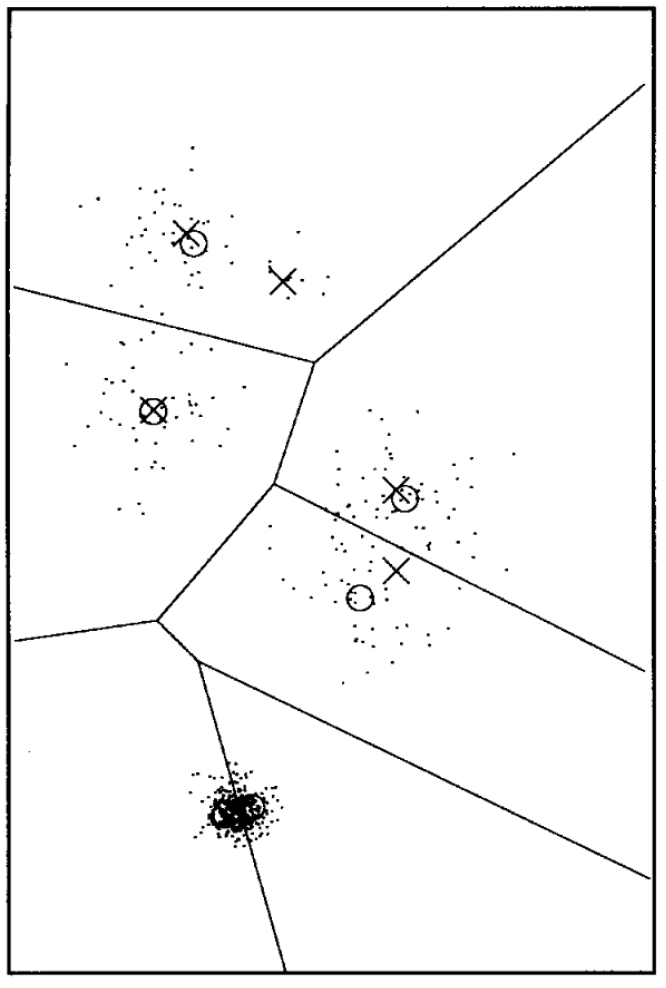
\includegraphics[width=\textwidth]{\dir/k_means_6}
        \caption{$K$-means}
        \label{fig:k_means_6}
    \end{subfigure}
    ~ %add desired spacing between images, e. g. ~, \quad, \qquad, \hfill etc. 
      %(or a blank line to force the subfigure onto a new line)
    \begin{subfigure}[b]{0.4\textwidth}
        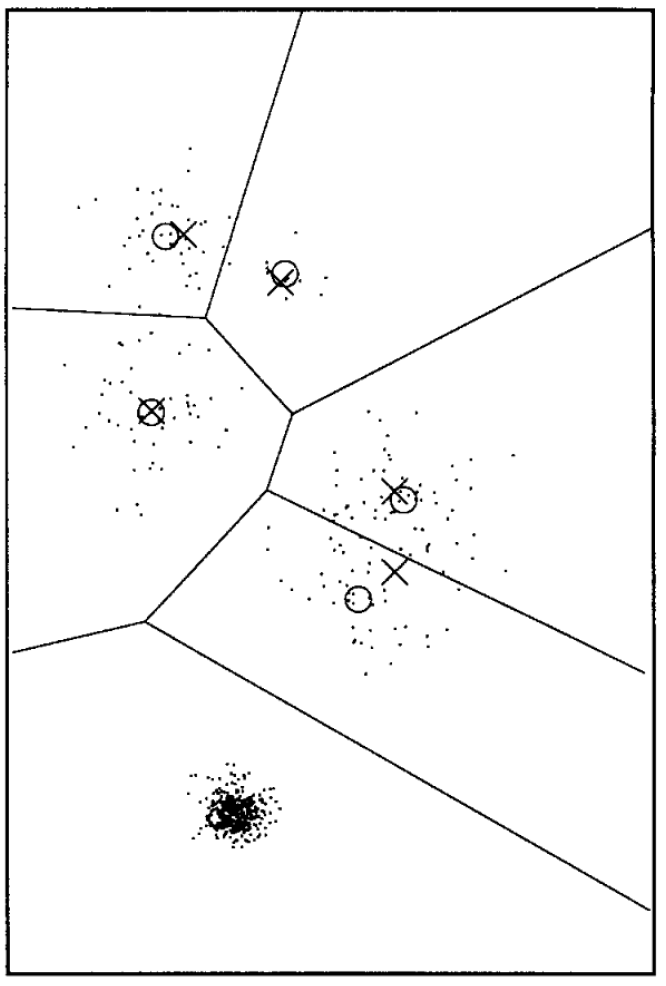
\includegraphics[width=\textwidth]{\dir/da_6}
        \caption{Deterministic annealing}
        \label{fig:da_6}
    \end{subfigure}
    \caption{Comparison of (a) $K$-means and (b) deterministic annealing. The $\times$ marks are the means of the Gaussian components. The $\bigcirc$ marks are the centroids computed by the algorithm.}
    \label{fig:da_vs_kmeans}
\end{figure}

\section{Phase transitions}
\label{sec:phase_transition}

We now study the behavior of the centroids as the temperature decreases.
We will see that, at the beginning when the temperature is high, all centroids
are equal to the sample mean. As a result one can assume that there
is only one cluster. As the temperature decreases, this cluster eventually decomposes into a few clusters, which continue decomposing into more clusters as the temperature keeps decreasing.

Figure~\ref{fig:da_phase_trans}, from Rose~\cite{rose1998deterministic}, illustrates this behavior. The four subfigures show the centroids ($\times$ marks) at four different points of the execution of
deterministic annealing with 9 centroids. Here, $X$ is a sample from a mixture of 9 Gaussians.
The subfigures are sorted by decreasing temperature. The curves in the graphic represent points that have all the same probability of belonging to one particular cluster. Observe how the apparent number of centroids change as the temperature
decreases. In Figure~\ref{fig:da_high_temp}, there seems to be only three centroids,
but what actually happens is that some of the 9 centroids are very close to
each other. Figure~\ref{fig:da_mid1_temp} shows the centroids after the temperature has decreased.
There seems to be now 5 centroids. In Figure~\ref{fig:da_mid2_temp} we have a lower
temperature and now 7 apparent centroids. Finally, in Figure~\ref{fig:da_low_temp}, all 9
centroids are at different locations and close to the means of the Gaussian
mixture.
We now investigate this behavior analytically. We do this through a
sequence of lemmas whose proofs are left as exercises.

\begin{figure}
    \centering
    \begin{subfigure}[b]{0.4\textwidth}
        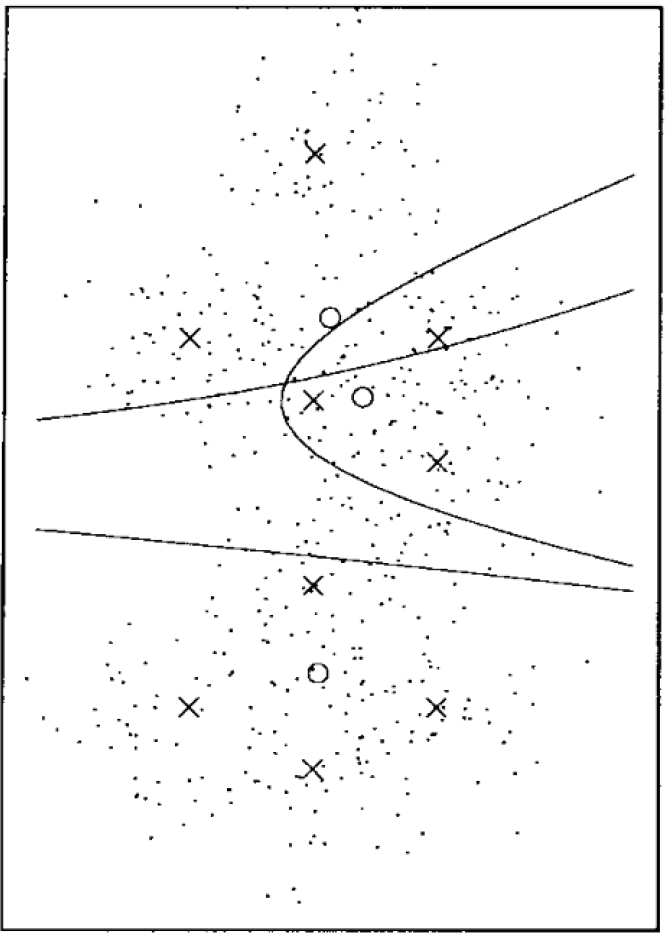
\includegraphics[width=\textwidth]{\dir/da_high_temp}
        \caption{}
        \label{fig:da_high_temp}
    \end{subfigure}
    ~ %add desired spacing between images, e. g. ~, \quad, \qquad, \hfill etc. 
      %(or a blank line to force the subfigure onto a new line)
    \begin{subfigure}[b]{0.4\textwidth}
        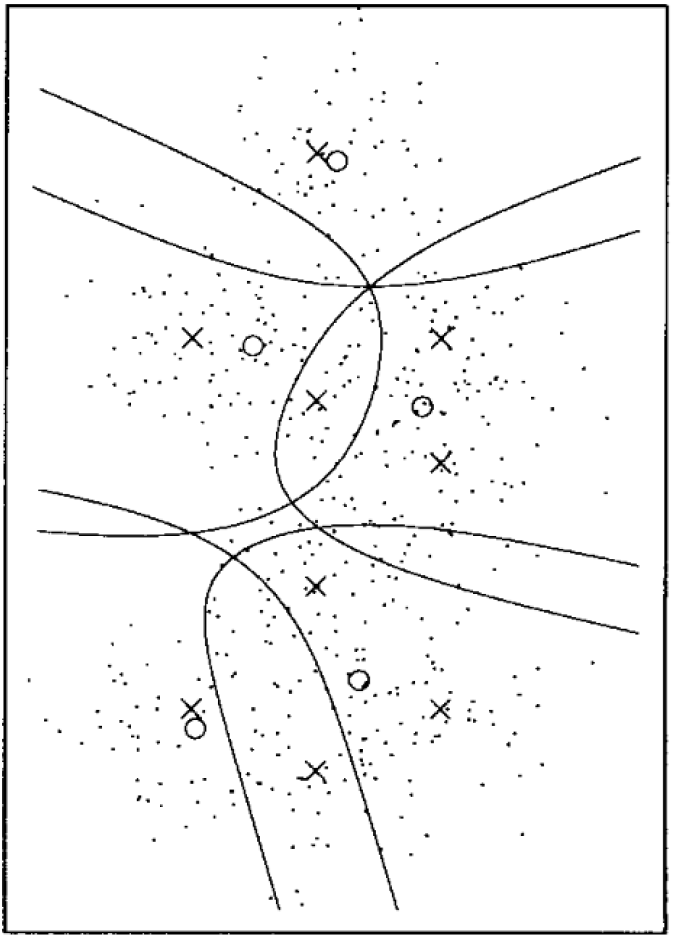
\includegraphics[width=\textwidth]{\dir/da_mid1_temp}
        \caption{}
        \label{fig:da_mid1_temp}
    \end{subfigure}
    
    \begin{subfigure}[b]{0.4\textwidth}
        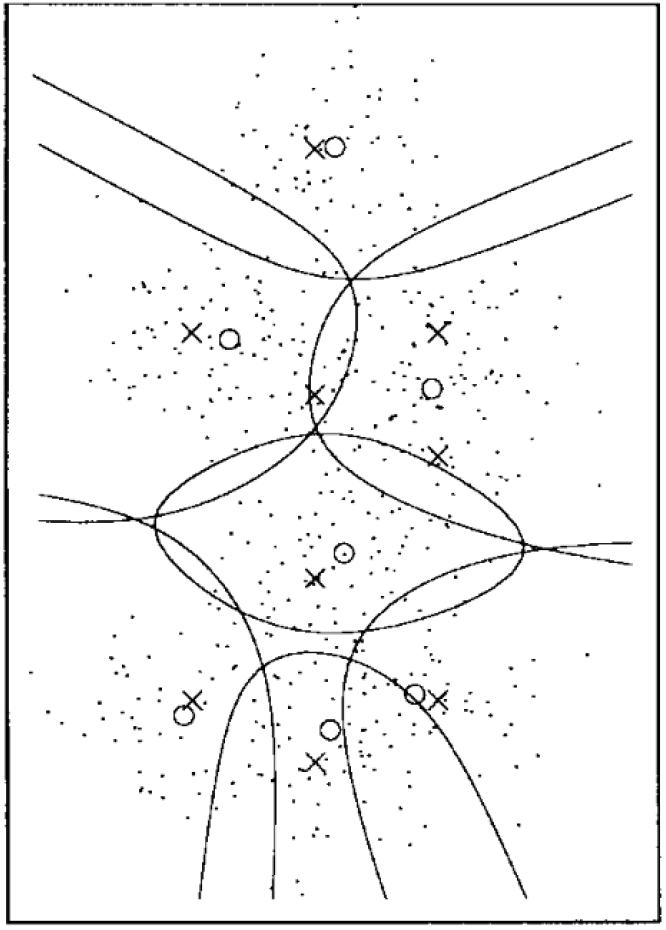
\includegraphics[width=\textwidth]{\dir/da_mid2_temp}
        \caption{}
        \label{fig:da_mid2_temp}
    \end{subfigure}
    ~ %add desired spacing between images, e. g. ~, \quad, \qquad, \hfill etc. 
      %(or a blank line to force the subfigure onto a new line)
    \begin{subfigure}[b]{0.4\textwidth}
        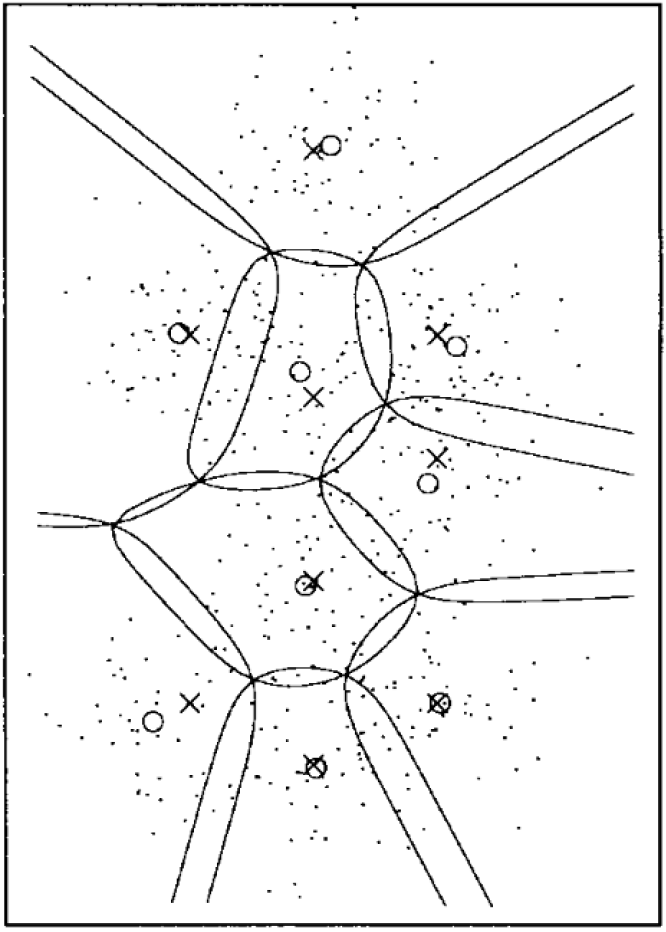
\includegraphics[width=\textwidth]{\dir/da_low_temp}
        \caption{}
        \label{fig:da_low_temp}
    \end{subfigure}
    \caption{}\label{fig:da_phase_trans}
\end{figure}

\subsection{There is only one cluster at a high temperature}

\begin{lemma}
\begin{equation}
\lim_{T \to \infty} \prob\left(C(i) = k \mid \theta, X\right) = \frac{1}{K}.
\end{equation}

\begin{equation}
\lim_{T \to 0} \prob\left(C(i) = k \mid \theta, X\right) = \begin{cases}
1 & \text{ if $\theta_k$ is the centroid closest to $x_k$ and}\\
0 & \text{ otherwise}.
\end{cases}
\end{equation}
\label{lem:da_extreme_temps}
\end{lemma}

\begin{proof}
This is a consequence of Exercise~\ref{ex:gibbs_dist_extreme_temps}.
\end{proof}

\begin{lemma}
For $R(\cdot, \theta, X)$, the $K$-means cost function, maximizing $H[p(\cdot \mid \theta, X)]$ with respect to $\theta$ is equivalent to minimizing
%
\begin{equation}
\mathcal{F}(\theta, X) := -T \sum_{i \leq N}\log \left(\sum_{k \leq K}\exp\left(-\frac{1}{T}\left\|x_i - \theta_{c(i)}\right\|^2\right)\right).
\label{eq:gibbs_free_energy_da}
\end{equation}
%
\label{lem:max_ent_is_min_free_energy_da}
\end{lemma}

\begin{proof}
The proof is similar to that of Lemma~\ref{lem:stationarity_condition} and involves Theorem~\ref{thm:gibbs_factorizes}.
\end{proof}

$\mathcal{F}\left(\theta, X\right)$ is called \emph{the Gibbs free energy (induced by $R(\cdot, \theta, X)$)}.

\begin{theorem}
At $T = 2\lambda$, there is a transition from one to several clusters, where $\lambda$ is the maximum eigenvalue of the sample covariance matrix of $X$. This is the matrix $\frac{1}{n}XX^\top$, where $X$ is seen as a matrix whose columns are all points in the observation.
\label{thm:critical_temp_da}
\end{theorem}

The rest of this section is devoted to prove lemmas that will help prove
this theorem.

Without loss of generality, we assume that $\theta^\infty = 0$. Observe that
when T is sufficiently high, the Hessian $H$ of $\mathcal{F}$ evaluated at $\theta^\infty$ is positive
definite. So new clusters arise when $H$ is no longer positive definite. Our plan is to demonstrate that $H$ stops being positive definite when $T = \frac{1}{2\lambda}$.

The Hessian $H$ can be seen as a block matrix where each block is the
Hessian matrix:
%
\begin{equation}
\frac{\partial F}{\partial \theta_\ell \partial \theta_k}\Bigr|_{\theta^\infty} = 
\left(
\begin{array}{ccc}
\displaystyle
\frac{\partial F}{\partial \theta_{\ell 1} \partial \theta_{k 1}}\Bigr|_{\theta^\infty} & \ldots & \displaystyle\frac{\partial F}{\partial \theta_{\ell 1} \partial \theta_{k d}}\Bigr|_{\theta^\infty}\\
\vdots & \ddots & \vdots\\
\displaystyle\frac{\partial F}{\partial \theta_{\ell d} \partial \theta_{k 1}}\Bigr|_{\theta^\infty} & \ldots & \displaystyle\frac{\partial F}{\partial \theta_{\ell d} \partial \theta_{k d}}\Bigr|_{\theta^\infty}
\end{array}
\right).
\end{equation}
%
From now on, we restrict the domain of $\frac{\partial F}{\partial \theta_\ell \partial \theta_k}$ to a ball $\mathcal{B}$ centered at the origin with a sufficiently small radius so that $\theta_k^\top \theta_\ell$ is insignificant, for every $k, \ell \leq K$. In particular, $\theta_{km}\theta_{\ell m'}$ is insignificant, for every $k, \ell \leq K$ and every $m, m' \leq d$.

\begin{lemma}
Inside $\mathcal{B}$,
%
\begin{equation}
\frac{\partial F}{\partial \theta_k} \approx -\frac{2}{T}\sum_{i \leq N} \frac{A_{ik}}{B_i},
\end{equation}
%
where
%
\begin{equation}
A_{ik} = (x_i - \theta_k)\left(1 + \frac{2}{T}x_i^\top \theta_i\right) \qquad \text{and} \qquad B_i = \sum_{k' \leq K}\left(1 + \frac{2}{T}x_i^\top \theta_{k'}\right).
\end{equation}
%
\label{lem:approx_deriv}
\end{lemma}

\begin{proof}
Start from
%
\begin{equation}
\frac{\partial F}{\partial \theta_k} = - \frac{2}{T} \sum_{i \leq N} \prob\left(C(i) = k \mid \theta, X\right)(x_i - \theta_k).
\label{eq:start_eq_da}
\end{equation}
%
Observe that, inside $\mathcal{B}$,
%
\begin{equation}
\left\|x_i - \theta_k\right\|^2 = \left\|x_i\right\|^2 - 2x_i^\top\theta_k + \left\|\theta_k\right\|^2 \approx \left\|x_i\right\|^2 - 2x_i^\top \theta_k.
\end{equation}
%
Hence,
%
\begin{align}
\exp\left(- \frac{1}{T}\left\|x_i - \theta_k\right\|^2\right) &\approx \exp\left(-\frac{1}{T}\left\|x_i\right\|^2\right)\exp\left(\frac{2}{T}x_i^\top \theta_k\right)\\
&\approx \exp\left(-\frac{1}{T}\left\|x_i\right\|^2\right)\left(1 + \frac{2}{T}x_i^\top \theta_k\right).\\
\end{align}
%
Therefore,
%
\begin{align}
\prob\left(C(i) = k \mid \theta, X\right) &= \frac{\exp\left(-\frac{1}{T}\left\|x_i - \theta_k\right\|^2\right)}{\sum_{k' \leq K}\exp\left(-\frac{1}{T}\left\|x_i - \theta_{k'}\right\|^2\right)}\\
&\approx \frac{\exp\left(-\frac{1}{T}\left\|x_i\right\|^2\right)\left(1 + \frac{2}{T}x_i^\top \theta_k\right)}{\sum_{k' \leq K}\exp\left(-\frac{1}{T}\left\|x_i\right\|^2\right)\left(1 + \frac{2}{T}x_i^\top \theta_{k'}\right)}\\
&= \frac{\left(1 + \frac{2}{T}x_i^\top \theta_{k}\right)}{\sum_{k' \leq K}\left(1 + \frac{2}{T}x_i^\top \theta_{k'}\right)}.\label{eq:simplified_factor_prob}
\end{align}
%
The result follows from plugging (\ref{eq:simplified_factor_prob}) in Equation~(\ref{eq:start_eq_da}).
\end{proof}

\begin{lemma}
\begin{equation}
\frac{\partial F}{\partial \theta_\ell \partial \theta_k}\Bigr|_{\theta^\infty} = \underbrace{\frac{2N}{K}\mathbb{I}\left\{\ell = k\right\}\left(I - \frac{2}{TN}XX^\top\right)}_{P} + \underbrace{\frac{2}{K^2}XX^\top.}_Q
\end{equation}
Here, $\mathbb{I}\left\{\ell = k\right\}$ is the identity matrix when $\ell = k$ and the zero matrix otherwise.
\end{lemma}

\begin{proof}
For $m, m' \leq d$, apply the quotient rule to show that
%
\begin{equation}
\frac{\partial F}{\partial \theta_{\ell m'} \partial \theta_{k m}}\Bigr|_{\theta^\infty}
=
-2\sum_{i \leq N}\left(\frac{1}{B_i}\Bigr|\frac{\partial A_{ikm}}{\partial \theta_{\ell m'}}\Bigr|_{\theta^\infty}\right) + 2 \sum_{i \leq N} \frac{A_{ikm}\Bigr|_{\theta^\infty}}{\left(B_i \Bigr|_{\theta^\infty}\right)^2}\left(\frac{\partial B_i}{\partial \theta_{\ell m'}}\Bigr|_{\theta^\infty}\right).
\end{equation}
%
Observe now that
%
\begin{equation}
A_{ik}\Bigr|_{\theta^\infty} = x_i, \quad B_i \Bigr|_{\theta^\infty} = K, \quad \text{and} \quad \frac{\partial B_i}{\partial \theta_\ell}\Bigr|_{\theta^\infty} = x_i.
\end{equation}
%
Therefore,
%
\begin{equation}
\frac{\partial F}{\partial \theta_{\ell} \partial \theta_{k}}\Bigr|_{\theta^\infty}
= - \frac{2}{K}\left(\frac{\partial}{\partial \theta_\ell}\sum_{i \leq N}A_{ik}\right)\Bigr|_{\theta^\infty} + \frac{2}{K^2}\sum_{i \leq N}x_i x_i^\top.
\label{eq:estimate_hessian_da}
\end{equation}
%
Show now that
%
\begin{equation}
\sum_{i \leq N}A_{ik} = \left(\frac{2}{T}XX^\top - NI\right)\theta_k.
\end{equation}
%
This implies that
%
\begin{equation}
\left(\frac{\partial}{\partial \theta_\ell}\sum_{i \leq N}A_{ik}\right)\Bigr|_{\theta^\infty} = N\mathbb{I}\left\{\ell = k\right\}\left(\frac{2}{TN}XX^\top - I\right).
\end{equation}
%
Plugging this into Equation~\ref{eq:estimate_hessian_da} yields the desired result.
\end{proof}

Observe that, with high probability, $Q$ is positive semi-definite.

\begin{lemma}
Let $Q$ be a positive semi-definite matrix. Let $H$ be a block
matrix where the block $(i,j)$ is given by
%
\begin{equation}
H[i,j] = \mathbb{I}\left\{\ell = k\right\} P + Q.
\end{equation}
%
Then $H$ is positive-definite iff $P$ is.
\label{lem:aux_lemma_ross}
\end{lemma}

\begin{proof}
See Rose's doctoral thesis~\cite{rose1991deterministic}.
\end{proof}

We now prove Theorem~\ref{thm:critical_temp_da}. Recall that the temperature at which $\theta^\infty$ stops being the unique minimum is the temperature at which the Hessian matrix $H$ evaluated at $\theta^\infty$ stops begin positive definite. By Lemma~\ref{lem:aux_lemma_ross}, this occurs when 
%
\begin{equation}
P = I - \frac{2}{TN}XX^\top
\end{equation}
%
is no longer positive definite, which occurs when
%
\begin{equation}
0 = \left|I - \frac{2}{TN}XX^\top\right| = \left|\frac{T}{2}I - \frac{1}{N}XX^\top\right|.
\end{equation}
%
That is, when $T/2$ is an eigenvalue of $\frac{1}{N}XX^\top$. Since $R$ starts at a very
large value and is gradually decreased, we conclude that the temperature at
which more clusters appear is at $T = 2\lambda$ where $\lambda$ is the largest eigenvalue of $\frac{1}{N}XX^\top$. This concludes the proof.

\section{Deterministic annealing and posterior agreement}
\label{sec:da_pa}

There is still an open question regarding deterministic annealing. What
is the number of clusters that we should use? More generally, at which
temperature we should stop the execution of deterministic annealing? The
posterior agreement principle recommends to have two observations $X'$ and
$X''$ and compute the temperature that maximizes the posterior agreement
kernel
%
\begin{equation}
\kappa(X', X'') = \sum_c p(c \mid X') p(c \mid X'').
\end{equation}
%
Observe that for the two probabilities to make sense, we must have $X' = \{x'_1, \ldots, x'_M\}$ and $X'' = \{x''_1, \ldots, x''_N\}$ of equal size. We assume from
now on that this is the case. Furthermore, we assume that $x'_i$ and $x''_i$, for $i \leq N$, are
two observations of one same object. The more general scenario is studied
by Buhmann~\cite{buhmann2010information}.

An analytical method to maximize $\kappa(X', X'')$ with respect to the temperature
is unknown. Moreover, the posterior agreement kernel seems to
be computationally intractable, as it is a sum over $K^N$ objects. Fortunately,
the factorization of the Gibbs distribution makes it computationally
tractable.

\begin{exercise}
Show that
%
\begin{equation}
\sum_{c}p(c \mid X') p(c \mid X'') = \prod_{i \leq N}\sum_{k \leq K}\prob\left(C(i) = k \mid X'\right)\prob\left(C(i) = k \mid X''\right).
\end{equation}
%
Show also that computing this takes $O(NK)$-time.
\end{exercise}

Our plan is then to select a set of candidate temperatures and pick the
one with the highest $\kappa(X', X'')$ as the stopping temperature. We can implement
this plan during the execution of deterministic annealing. Observe
that the while loop of of Algorithm~\ref{algo:da_algo_da} gives as a sequence of decreasing
temperatures. Therefore, we can compute $\kappa(X', X'')$ at each iteration
with the current temperature. We can keep track of these kernel values.
The value of $\kappa(X', X'')$ has been observed empirically to be low when the
temperature is high, then it increases as the temperature is lowered, and
eventually it starts decreasing. Hence, we can keep track of how the kernel
values change as deterministic annealing decreases the temperature. After
observing, for a certain amount of iterations, that $\kappa(X', X'')$ is no longer
increasing and starts decreasing, we can stop the annealing and choose as
stopping temperature the one that yielded the largest $\kappa(X', X'')$.